\section{Data Conditioning}
\label{sec:conditioning}

\lorena{The training and testing data represent $\sim 200,000$ binary systems comprised
of binary neutron stars (BNS), neutron star-black hole (NSBH), and binary black 
hole (BBH) systems. The data is divided into a training/testing breakdown of
$70\%/30\%$. Regression is applied to four features, namely the initial masses
$m_1$ and $m_2$ and initial spin magnitudes $\chi_1$ and $\chi_2$. Injections are carried
through using LIGO's second observing run (O2) and recovered using the
\texttt{GstLAL} pipeline. This low-latency pipeline uses matched-filtering 
techniques for the detection of gravitational-wave signals from compact
binaries. The instrinsic parameters of the best-fit template are then given as
possible true parameters of the system. However, these parameters may not be
the actual parameters of the astrophysical system due in part to waveform 
systematics but mainly due to detector noise. For a detection, slower but 
more accurate parameter estimation is conducted using different codes like
\texttt{LALInference} and \texttt{Bilby}, among others. However, it is
important to have an estimate of parameters in low latency. Moreover, a single 
astrophysical event, or injection in our case, may ring multiple triggers 
corresponding to different templates. This may add a layer of complication.
(Mention approximants used?) The training dataset has mass ranges 
$m_1 =  [1.02, 116]$ and $m_2 =  [0.81, 81]$ and spin ranges 
$\chi_{1,2} =  [-0.99, 0.99]$, as shown in 
Fig.~\ref{parameter_space}.}

\begin{figure}
	\centering
	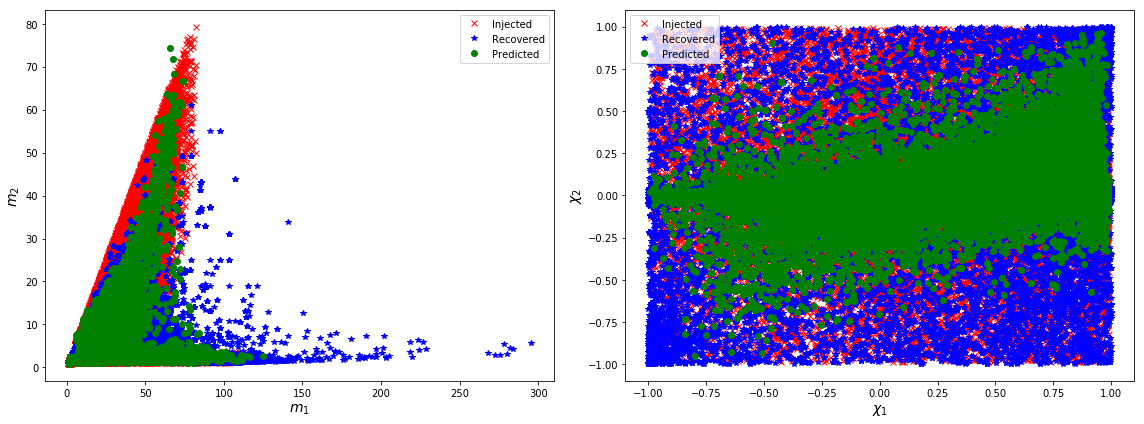
\includegraphics[width=0.45\textwidth]{m1m2_chi1chi2_comparison.png}
    \caption{\lorena{The $m_1$-$m_2$ (left) and $\chi_1$-$\chi_2$ (right) parameter space 
		of injections is shown in red, the recovered
  		values from matched-filtering are in blue, and the predicted values from 
        regression are in green.}}
	\label{parameter_space}
\end{figure}

\lorena{We prepare the data for regression in three steps:}
\begin{enumerate}[label=(\roman*)]
    \item \lorena{First, we map the data to be in the range from $(0,1)$. We do
            this by solving a simple, linear system of equations separately for 
            the masses and the spins since they span different ranges of
            values.}
    \item \lorena{Second, we map the data to be in the range from
        $(-\infty,+\infty)$. We do this to ensure positive values in mass and
        spin predictions. Otherwise, results are unphysical. This mapping
        requires the previous $(0,1)$ mapping of the data.}
    \item \lorena{Finally, we standardize the data to have a zero mean and unit 
        variance.}
\end{enumerate}

\lorena{Once the algorithm gives us the predicted data, the reverse process is
done, i.e., the data is scaled back from standardization, mapped back to 
$(0,1)$, and exponentiated.}
